\documentclass[conference]{IEEEtran}
\usepackage{amsmath,amssymb}
\usepackage{graphicx}
\usepackage{booktabs}
\usepackage{tikz}
\usetikzlibrary{shapes,arrows.meta,positioning,fit}
\usepackage{pgfplots}
\pgfplotsset{compat=1.18}
\usepackage{siunitx}
\usepackage{multirow}
\usepackage{hyperref}

\newcommand{\eg}{e.g.}
\newcommand{\ie}{i.e.}

\begin{document}

\title{An LLM-Orchestrated DC--DC Converter Design Platform with a
Deterministic Physics Engine: Architecture and Hardware Validation of
\texttt{pyspice\_openfoam\_agent}}

\author{\IEEEauthorblockN{Pyspice-Openfoam-Agent Project}
\IEEEauthorblockA{Repository: github.com/abdul-basit-ai/Pyspice-Openfoam-agent}}

\maketitle

\begin{abstract}
Manual DC--DC converter design couples electrical synthesis, circuit
simulation, loss modeling, and thermal analysis in a slow, error-prone
loop, while large language models (LLMs) used alone hallucinate part
numbers and physics. This report documents \texttt{pyspice\_openfoam\_agent},
a platform that resolves the tension by architectural separation: an LLM
agent (LangGraph ReAct, OpenRouter/DeepSeek) orchestrates, but every
physics number --- margins, losses, temperatures, efficiencies --- is
produced by deterministic, unit-tested engineering code (PySpice/ngspice,
python-control, OpenFOAM, NSGA-II). The pipeline spans specification
parsing, topology synthesis, real-component selection, netlist synthesis,
transient SPICE with steady-state detection, topology-aware loss
extraction, Type~III control-loop design, conjugate-heat-transfer (CHT)
simulation, and multi-objective optimization, bound by a system-wide
best-effort contract: bounded convergence first, closest-achievable
result with an explicit caveat otherwise --- never a silent pass. The
physics engine is validated against real TI evaluation-module (EVM)
hardware: on a synchronous buck EVM (LM27402) the engine tracks measured
efficiency with a mean absolute error of \SI{0.22}{pp} over 17 matched
load points; a buck-boost EVM validates with a documented, currently
unexplained residual (MAE \SI{2.47}{pp}); no qualifying boost EVM was
found. Component selection is out of scope; parts are injected.
\end{abstract}

\section{Introduction}
Designing a switching power converter requires iterating across
electrical synthesis, component selection, circuit simulation, loss
accounting, and thermal verification. Each iteration is manual,
slow, and dependent on expert judgment; small errors (a stale loss
constant, a missed dead-time effect) silently propagate into operating
points that real hardware does not meet. LLM assistants promise to
accelerate this loop, but used as the calculator they are unsafe: they
invent part numbers, guess margins, and present fabricated physics with
fluency.

The core design principle of this project is therefore a strict division
of labor: \emph{the LLM never computes a margin and never invents a part
number}. Every physics number comes from deterministic, unit-tested
engineering code --- SPICE transients, python-control frequency analysis,
OpenFOAM CHT solves, NSGA-II optimization. The LLM's role is
orchestration: parsing intent, choosing tools, interpreting results,
and recovering from errors, all auditable through logged prompts and
responses. The project's own engineering policies codify where the agent
must ask the user rather than guess (\eg\ efficiency-versus-cost,
cooling type, optimization objective)~\cite{goals}.

This report documents the resulting system end to end: architecture
(Section~\ref{sec:arch}), the engineering decisions that shaped it and
what the audit caught in practice (Section~\ref{sec:decisions}), the
hardware-validation methodology (Section~\ref{sec:method}), results
against real TI evaluation modules (Section~\ref{sec:results}), and the
limitations that remain open (Section~\ref{sec:limits}).

\section{System Architecture}
\label{sec:arch}

The pipeline follows the phase dependency map of the project's goals
document~\cite{goals}: a specification is parsed into structured
requirements (Phase~2), screened for feasibility, and mapped to one of
three supported topologies --- synchronous buck, synchronous boost, and
4-switch non-inverting buck-boost --- with analytical inductor and
capacitor sizing (Phase~3). A unified design object (Phase~4) is the
single source of truth; schematics, netlists, bills of material, and
reports all generate from it. Margin-based selection picks real
components from a curated library (Phase~5); the netlist synthesizer
emits SPICE with an ngspice lint and connectivity validation. A
deterministic control-loop stage (Phase~6) designs a Type~III
compensator and computes phase and gain margins; these are never
LLM-judged. Transient SPICE simulation (Phase~8) with cycle-to-cycle
steady-state detection feeds topology-aware loss extraction
(Phase~9). Losses drive a reduced-order electro-thermal fixed point and,
on demand, a full 3D OpenFOAM CHT solve on a JEDEC-style board
(Phases~10--13), with the CHT solve running
chtMultiRegionSimpleFoam~\cite{openfoam}. NSGA-II multi-objective
optimization (Phase~14) via pymoo~\cite{pymoo} evaluates candidates with
the reduced-order model and verifies finalists with full CHT.
Fig.~\ref{fig:arch} shows the main stages and the electro-thermal
convergence loop.

\begin{figure*}[t]
\centering
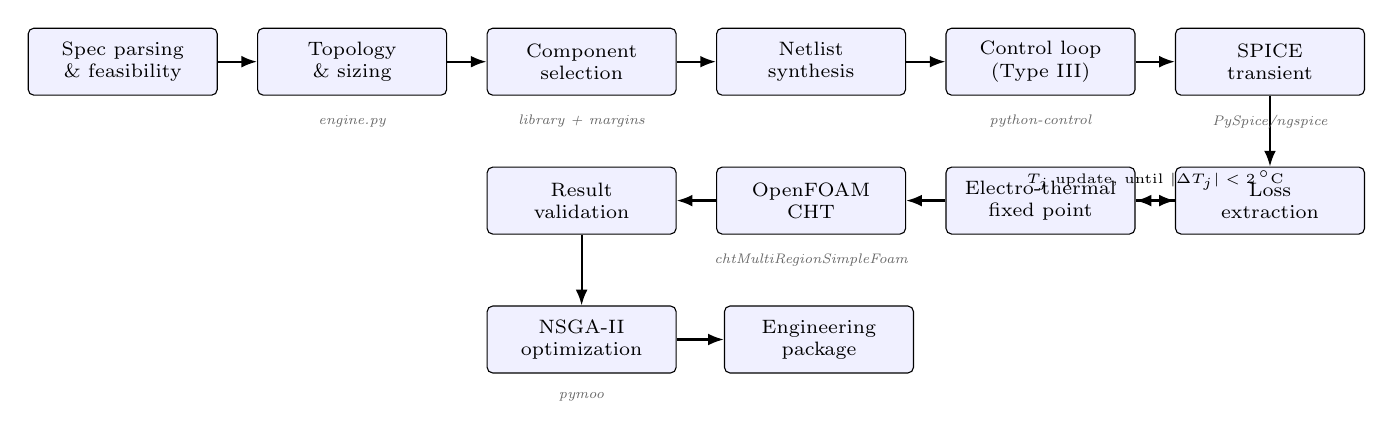
\begin{tikzpicture}[
  stage/.style={draw, rounded corners=2pt, align=center, minimum height=8.5mm,
                minimum width=24mm, font=\scriptsize, fill=blue!6},
  tool/.style={font=\tiny\itshape, text=black!60, align=center},
  arr/.style={-{Latex[length=2mm]}, thick},
  node distance=4mm and 5mm]
\node[stage] (spec) {Spec parsing\\ \& feasibility};
\node[stage, right=of spec] (size) {Topology\\ \& sizing};
\node[stage, right=of size] (select) {Component\\ selection};
\node[stage, right=of select] (net) {Netlist\\ synthesis};
\node[stage, right=of net] (ctrl) {Control loop\\ (Type III)};
\node[stage, right=of ctrl] (spice) {SPICE\\ transient};
\node[stage, below=9mm of spice] (loss) {Loss\\ extraction};
\node[stage, left=of loss] (et) {Electro-thermal\\ fixed point};
\node[stage, left=of et] (cht) {OpenFOAM\\ CHT};
\node[stage, left=of cht] (val) {Result\\ validation};
\node[stage, below=9mm of val] (opt) {NSGA-II\\ optimization};
\node[stage, right=6mm of opt] (pkg) {Engineering\\ package};
\draw[arr] (spec) -- (size);
\draw[arr] (size) -- (select);
\draw[arr] (select) -- (net);
\draw[arr] (net) -- (ctrl);
\draw[arr] (ctrl) -- (spice);
\draw[arr] (spice) -- (loss);
\draw[arr] (loss) -- (et);
\draw[arr] (et) -- (cht);
\draw[arr] (cht) -- (val);
\draw[arr] (val) -- (opt);
\draw[arr] (opt) -- (pkg);
% electro-thermal loop-back (goals doc: Phase 13 -> Phase 9)
\draw[arr, dashed] (et) -- node[above, font=\tiny, sloped] {$T_j$ update, until $|\Delta T_j|<2\,^\circ$C} (loss);
% tool annotations
\node[tool, below=1.2mm of size] {engine.py};
\node[tool, below=1.2mm of select] {library + margins};
\node[tool, below=1.2mm of ctrl] {python-control};
\node[tool, below=1.2mm of spice] {PySpice/ngspice};
\node[tool, below=1.2mm of cht] {chtMultiRegionSimpleFoam};
\node[tool, below=1.2mm of opt] {pymoo};
\end{tikzpicture}
\caption{Main pipeline stages (top row, left to right), thermal path and
optimizer (bottom row). The dashed arrow is the electro-thermal
convergence loop: the newly converged $T_j$ updates device temperatures
and losses re-extract until $|\Delta T_j| < 2\,^\circ$C (bounded at 8
iterations; non-convergence is reported as a validation failure). Tool
names under each stage are the deterministic engines that produce the
numbers. Stage order follows the phase dependency
map~\cite{goals}.}
\label{fig:arch}
\end{figure*}

The orchestrator is a LangGraph ReAct loop~\cite{langgraph}: the agent
reasons, calls one tool at a time, and observes the compact result. The
tool contract enforces the architecture's safety property from both
sides. Tools return compact dictionaries (numbers and status), never raw
waveforms or VTK dumps, so LLM context stays small; tool errors are
returned as structured \texttt{\{"error": ...\}} dictionaries rather
than exceptions, so the agent observes failures and recovers instead of
crashing. The component library is the only source of parts: the agent
may select among parts returned by library queries and must never
invent a part number or rating. Every design-decision LLM call logs
model, temperature (zero), full prompt and response to a provenance
file, and each run persists the design object, a run manifest, and the
provenance trail. A design-memory store records completed designs keyed
by specification signature and feeds the best-known configuration to
future runs.

\section{Key Engineering Decisions}
\label{sec:decisions}

\subsection{Deterministic tools for physics, LLM for orchestration}
The hallucination guardrail is structural, not advisory. Margins are
computed by python-control/scipy from the analytic plant; losses by a
topology-aware extraction from simulated waveforms; junction
temperatures by the fixed-point loop or CHT. Where the LLM produces
text (\eg\ the final design summary), the system separately enforces
verdict integrity: every tool failure observed during a run is attached
to the summary as a caveat and rendered as a banner, so the agent
cannot bury a failure under fluent prose.

\subsection{The duty servo}
An open-loop SPICE rig at the nominal duty always sits below the design
output voltage by the static drops (dead-time diode clamp, inductor DCR,
switch on-resistance) --- exactly what a closed-loop controller
compensates in hardware. Rather than report the wrong operating point,
\texttt{run\_spice} runs a bounded deterministic duty servo: it probes
the rig, brackets the target output voltage, seeds the search with
volt-second balance, and converges with damped secant/bisection steps
inside the renderable trim range. The audited result: buck converged to
4.97~V, boost and buck-boost within 0.5\% of target, with servo
provenance recorded in the artifacts and netlist header
\cite{audit}.

\subsection{Electro-thermal fixed point}
Losses depend on junction temperature (on-resistance rises with $T_j$),
and $T_j$ depends on losses. The loop alternates loss extraction and a
thermal estimate from a converged seed, with adaptive damping
(relaxation halves when the residual grows) and a bound of 8 iterations;
convergence requires $|\Delta T_j| < 2\,^\circ$C and non-convergence is
error-tagged, never accepted silently. The per-topology conduction
factor (buck exactly $D+(1-D)$; boost and buck-boost carry
$I_{out}/(1-D)$ through the switches) replaced an earlier blanket
1.5$\times$ factor that was wrong for every topology. The loop also
honestly reports thermal runaway: for linearized loop gain $\geq 1$ no
positive fixed point exists \cite{audit}.

\subsection{The best-effort contract}
A deliberate system-wide principle (user-directed) is that every stage
tries bounded, deterministic convergence first and degrades to the
closest achievable result with an explicit caveat --- never a silent
pass, never a dead end. Ripple misses trigger a duty servo, then
capacitor banking, then auto-upsizing, each re-simulated; an
electro-thermal non-convergence returns the last damped estimate tagged
\emph{thermally suspect}; a CHT overshoot auto-triggers mitigation
(airflow, reselection, frequency) and returns the best mitigated
configuration with a caveat. All caveats funnel into the run summary.
This is what makes the system usable by a non-expert: the pipeline
cannot fail invisibly \cite{audit}.

\subsection{What the audit caught}
A full audit \cite{audit} traced every finding to root cause, fix, and
verification, with regression tests pinning each one. Two
consequential examples:

\emph{Dead-time inconsistency.} A hardening change had set the gate
dead time to \SI{152}{ns} (7.6\% of a \SI{500}{kHz} period, three dead
windows per cycle) while the loss model still assumed \SI{30}{ns}. The
rig sat $\sim$22\% below the target output voltage and every downstream
number --- offset health gate, losses, efficiency --- was taken at the
wrong operating point. The fix made \texttt{dead\_time\_for()} the
single source of truth (\SI{30}{ns} minimum, twice the modeled
crossover), imported it into the loss model, and modeled the three dead
windows the gate phasing actually opens.

\emph{CHT log overwrite masked divergence.} Each OpenFOAM relaxation
attempt overwrote the solve log, destroying divergence evidence, and
success was declared on a return code plus a NaN count that the
validator (any NaN = invalid) was guaranteed to reject. The fix
preserves per-attempt logs, fails on any NaN, checks that the solver
reached its end time, and under-relaxes solid-region energy equations
in the retry ladder.

The audit also found a capacitor ESL modeling error that injected
$\pm$40~V non-physical spikes into the rig (removed; ESL is
milliohms at the switching frequency), a Pareto optimizer that ranked
every topology with buck physics (fixed per-topology), and a
PWM-delay error that overstated phase margin by roughly 18 degrees at
the buck crossover (fixed with an all-pass delay term and a
phase-targeted Type~III design).

\section{Validation Methodology}
\label{sec:method}

The physics engine is validated against real, published TI evaluation
modules. The methodology, from \cite{valreport}:

\textbf{EVM-exact injection.} Component selection is explicitly out of
scope: every run injects the EVM's exact power-path parts and bypasses
the selector, so validation isolates the physics engine from the
selection logic. Every injected field carries a source flag ---
\emph{published} (datasheet/BOM), \emph{derived} (computed, derivation
shown), \emph{pipeline\_estimate} (documented, listed as an unmatched
factor, sensitivity stated), or \emph{sentinel} (schema-required but
unused by the simulated physics, so it cannot influence any number).

\textbf{Digitized measurement with stated uncertainty.} The measured
efficiency curve is digitized from the vector figure in the EVM user's
guide with a stated $\pm\SI{0.3}{pp}$ uncertainty floor under every
error claim.

\textbf{Matched-point simulation.} The pipeline runs at every matched
load point; the pipeline is deterministic at fixed load, so a single
run per point suffices.

\textbf{Error convention.} Error $=$ simulated $-$ measured, in
percentage points. \emph{Positive} error means the simulator claims
better efficiency than the real board delivers --- the optimistic,
dangerous direction, reported separately from under-prediction, which
is conservative.

\section{Results}
\label{sec:results}

Table~\ref{tab:summary} summarizes the three-topology outcome;
Fig.~\ref{fig:buck} shows the buck per-load comparison.

\begin{table}[t]
\centering
\caption{Validation summary across topologies (from \cite{valreport}).
Error convention: sim $-$ measured; positive is optimistic.}
\label{tab:summary}
\begin{tabular}{llSSl}
\toprule
Topology & EVM & {MAE (pp)} & {Worst (pp)} & Bias direction \\
\midrule
boost & not found & {---} & {---} & --- \\
buck & LM27402 & 0.22 & {+0.81} & optimistic \\
buck-boost & LM5175EVM-HD & 2.47 & {$-2.97$} & conservative \\
\bottomrule
\end{tabular}
\end{table}

\begin{figure}[t]
\centering
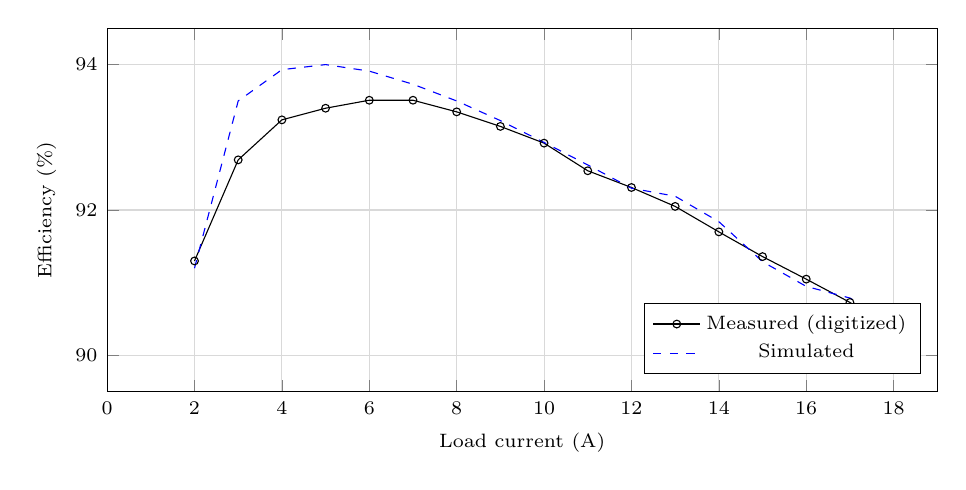
\begin{tikzpicture}
\begin{axis}[
  width=\columnwidth, height=6.2cm,
  xlabel={Load current (A)}, ylabel={Efficiency (\%)},
  xmin=0, xmax=19, ymin=89.5, ymax=94.5,
  legend style={font=\scriptsize, at={(0.98,0.05)}, anchor=south east},
  tick label style={font=\scriptsize}, label style={font=\scriptsize},
  grid=both, grid style={black!15}]
\addplot[mark=o, mark size=1.4pt, black] coordinates {
 (2,91.30) (3,92.69) (4,93.24) (5,93.40) (6,93.51) (7,93.51)
 (8,93.35) (9,93.15) (10,92.92) (11,92.54) (12,92.31) (13,92.05)
 (14,91.70) (15,91.36) (16,91.05) (17,90.73) (18,90.34)};
\addlegendentry{Measured (digitized)}
\addplot[mark=s, mark size=1.4pt, blue, dashed] coordinates {
 (2,91.20) (3,93.50) (4,93.93) (5,94.00) (6,93.91) (7,93.73)
 (8,93.50) (9,93.23) (10,92.93) (11,92.62) (12,92.30) (13,92.19)
 (14,91.84) (15,91.29) (16,90.95) (17,90.79) (18,90.44)};
\addlegendentry{Simulated}
\end{axis}
\end{tikzpicture}
\caption{Buck validation, LM27402 EVM (\SI{12}{V} $\rightarrow$
\SI{1.5}{V}, \SI{300}{kHz}): measured vs.\ simulated efficiency over 17
matched load points. MAE \SI{0.22}{pp}; worst point $+0.81$~pp at
\SI{3}{A}. Data from \cite{valreport}.}
\label{fig:buck}
\end{figure}

\textbf{Buck (LM27402 EVM, \cite{snva406}).} MAE \SI{0.22}{pp} over 17
matched loads; worst $+0.81$~pp at \SI{3}{A}. The bias skews optimistic
at light load: 13 of 17 points over-predict, mean $+0.27$~pp. A
sensitivity check perturbed the estimated MOSFET plateau voltage by
$\pm$20\%: it moves the \SI{3}{A} error by only $\sim\pm 0.15$~pp and
cannot close the light-load gap, ruling the plateau estimate out as the
dominant driver; the consistent remaining explanation is the omitted
loss terms (reverse recovery, high-side output capacitance,
controller/gate quiescent consumption) that the behavioral rig does not
model.

\textbf{Buck-boost (LM5175EVM-HD, \cite{snvu439}).} MAE \SI{2.47}{pp}
over 10 matched loads, uniformly conservative (every point
under-predicts, worst $-2.97$~pp at \SI{5.5}{A}). Injecting the EVM's
per-leg switch parts exactly as the BOM (one part on leg~1, another on
leg~2, replacing a single part on all four switches) recovered only
2.66~$\rightarrow$~2.47~pp --- not the $\sim$1~pp predicted from the
leg-2 conduction analysis. The real board is unusually efficient
($\approx$98.3\%) at its 12~V transition point, and the residual is
\emph{not explained}: recorded as an open question with unconfirmed
candidate causes (the behavioral gate-drive model, omitted
reverse-recovery on the low-side parts, first-order crossover-loss
assumptions in this switching regime). We report it as unresolved.

\textbf{Boost.} Not validated. After a genuine search across TI, ADI,
and onsemi, no single-phase \emph{discrete-FET} synchronous boost EVM
was found with schematic, BOM, a digitizable efficiency curve, and
stated conditions; available candidates use integrated GaN power stages
(no defensible mapping onto a discrete-MOSFET schema) or are
dual-phase. This is stated as an explicit negative result rather than a
silently-open gap.

\section{Limitations and Future Work}
\label{sec:limits}

The validated claims are narrow, and the project's own documents say
so~\cite{valreport,goals}:
\begin{itemize}
\item \textbf{Component selection is not validated} --- parts are
injected, not selected; selection logic is exercised by the unit suite
only.
\item \textbf{One EVM per topology, one operating-point sweep per EVM}:
the engine is validated at the measured points, not across the full
input/frequency design space.
\item \textbf{No thermal validation on any processed EVM}: the source
user's guides do not state ambient or airflow conditions, so no
temperature comparison is claimed anywhere.
\item \textbf{The buck-boost residual is unresolved} (Section~\ref{sec:results});
the \SI{2.47}{pp} number is not understood or bounded.
\item \textbf{Boost is not yet validated}; a qualifying EVM is future
work if one becomes available.
\item \textbf{Closed-loop SPICE} (a behavioral or physical Type~III
network inside the netlist) was explored and is blocked by a
shared-library ngspice limitation; the compensated loop is validated by
deterministic margin analysis and open-loop step tests only
\cite{goals}.
\item \textbf{Known model heuristics}: first-order crossover-loss model
with clamps; conservative blocking voltage on the buck-boost output
pair; core-loss modeling required for electro-thermal convergence is a
library-data gap; hardware-in-the-loop validation (Phase~21) is
deliberately deferred until physical hardware exists \cite{goals}.
\end{itemize}

\section{Conclusion}
The project demonstrates that an LLM-orchestrated design platform can be
made safe for power-electronics engineering by architectural separation:
the agent orchestrates, deterministic and unit-tested engines compute.
On the validated topology and operating points, the physics engine
tracks real hardware to \SI{0.22}{pp} mean absolute error --- within
stated digitization uncertainty for most of the load range --- and every
deviation is either explained (buck light load, dominated by identified
omitted loss terms) or honestly recorded as open (buck-boost residual).
What is \emph{not} yet demonstrated is generalization: other topologies
(boost), wider operating ranges, component selection, thermal
predictions against hardware, and closed-loop simulation inside SPICE.
The value of the approach lies as much in what the audit and validation
process caught --- an inconsistent dead-time model, a masked CHT
divergence, a verdict that buried a failure --- as in the headline
number: the discipline of deterministic, traceable physics is what makes
both the errors and the honest reporting of them possible.

\begin{thebibliography}{9}

\bibitem{goals}
\emph{Advanced AI Power Electronics Design \& Multiphysics Platform ---
updated project goals (Phases 0--23)}, project document,
\texttt{updated\_project\_goals.md},
\texttt{github.com/abdul-basit-ai/Pyspice-Openfoam-agent}, 2026.

\bibitem{audit}
\emph{Project audit --- findings, fixes, verification},
project document, \texttt{AUDIT.md},
\texttt{github.com/abdul-basit-ai/Pyspice-Openfoam-agent}, 2026.

\bibitem{valreport}
\emph{Validation error report --- physics engine vs.\ TI EVM
measurements}, project document, \texttt{validation/error\_report.md}
and \texttt{validation/README.md},
\texttt{github.com/abdul-basit-ai/Pyspice-Openfoam-agent}, 2026.

\bibitem{snva406}
Texas Instruments, \emph{LM27402 Evaluation Module 12--V Input, 1.5--V
Output 20--A EVM User's Guide}, SNVA406C.

\bibitem{snvu439}
Texas Instruments, \emph{LM5175EVM-HD User's Guide}, SNVU439.

\bibitem{langgraph}
LangChain Inc., \emph{LangGraph: Building Stateful, Multi-Actor
Applications with LLMs}, \texttt{github.com/langchain-ai/langgraph}, 2024.

\bibitem{openfoam}
OpenCFD Ltd., \emph{OpenFOAM v2406 User Guide}, OpenFOAM Foundation /
OpenCFD, 2024.

\bibitem{pymoo}
J.~Blank and K.~Deb, ``pymoo: Multi-objective optimization in Python,''
\emph{IEEE Access}, vol.~8, 2020.

\end{thebibliography}

\end{document}
